\documentclass[11pt,a4paper]{report}

\usepackage[polish]{babel}
\usepackage[utf8x]{inputenc}
\usepackage{polski}
%\usepackage[T1]{fontenc}
\frenchspacing
\usepackage{indentfirst}
\usepackage{amsthm}
\usepackage{amsmath}
\usepackage{algorithmic}
\usepackage{algorithm}
\usepackage{program}
\usepackage{programs}
\usepackage{array}
\usepackage{multirow}
\usepackage{graphicx}
\usepackage{listings}
\usepackage{listing}
\usepackage{float}
\pagenumbering{arabic}

\graphicspath{{img/}}

\begin{document}
\tableofcontents
\listoflistings
\chapter{Preprocessing}

W aplikacji znajdują się trzy różne preprocessingi zebranych danych. Jeden służy szybszemu wyliczaniu informacji przy algorytmach Adapted Pagerank i Social Pagerank. Algorytmy te przy każdym przebiegu korzystają z tych wyliczanych danych. Obliczanie ich przy każdej iteracji wymagałoby dużego nakładu czasu. Drugie wyliczane dane używane są przy wyświetlaniu wyników i w czasie obliczenia ostatecznych ranków  poszczególnych dokumentów.

\section{Dane algorytmów}

Dane dla algorytmów wyliczane są w dwóch częściach. Na początku wyliczane są dane w bazie danych i zapisywane w bazie, następnie, po wyliczeniu zapisywane są one do do struktury i serializowane w plikach. Dane ze zserializowanych plików używane są później do tworzenia macierzy.

\subsection{Preprocessing w bazie danych}

W bazie danych wyliczone zostają informacje potrzebne do późniejszego utworzenia macierzy. Informacje te zostaną zapisane w tabeli USERTAGDOC w polu how\_much i w tabelach TAG\_USR i TAG\_DOC. Wyliczenie tych informacji pozwoli później na szybszy dostęp do nich i 

Czas wykonania preprocessingu w bazie danych jest różny. Jak widać w tabeli poniżej najwięcej czasu trwało tworzenie tabeli TAG\_USR i powstało w niej najwięcej nowych rekordów. Prawdopodobnie jest to spowodowane tym, że użytkownicy używają różnych tagów przy oznaczaniu różnych dokumentów. Z drugiej strony, dokumenty, mimo ze opisywane są przez różnych użytkowników, oznaczone są najczęściej podobnymi tagami.

\begin{center}
    \begin{tabular}{ | c | p{3cm}| p{3cm} | }
    \hline
    Tabela & czas wykonania polecenia & ilość powstałych rekordów  \\ 
    \hline
    TAG\_USR & 22h 34min 4s & 26,938,914   \\ 
    \hline
    TAG\_DOC & 3h 13min 23s  &  14,563,924\\ 
    \hline
    USERTAGDOC & 1h 34min 17s  & $14563924$  \\ 
    \hline
    \end{tabular}
\end{center}

Poniżej znajdują się listingi zapytań SQL updatujące tabele USRTAGDOC \ref{sql_usrtagdoc} i wypełniający tabele TAG\_USR (\ref{sql_tag_doc}) i TAG\_DOC (\ref{sql_tag_usr}). 


\lstset{language=SQL}   
\begin{lstlisting}[frame=lines, caption={Skrypt dodający dane do tabeli tag\_doc}, label={sql_tag_doc}]
insert into tag_doc (tag_id, doc_id, how_much)
select tag.id, utd.doc_id, 1
from
tag,
usertagdoc_tag as utd_t,
usertagdoc as utd
where
utd_t.usertagdoc_id = utd.id and
utd_t.tags_id = tag.id
on duplicate key update how_much=how_much+1;
\end{lstlisting}

\begin{lstlisting}[frame=lines, caption={Skrypt dodający dane do tabeli tag\_usr}, label={sql_tag_usr}]]
insert into tag_usr (tag_id, user_id, how_much)
select tag.id, utd.user_id, 1
from
tag,
usertagdoc_tag as utd_t,
usertagdoc as utd
where
utd_t.usertagdoc_id = utd.id and
utd_t.tags_id = tag.id
on duplicate key update how_much=how_much+1;
\end{lstlisting}

\begin{lstlisting}[frame=lines, caption={Skrypt updatujący pole how\_much w tabeli usertagdoc}, label={sql_usrtagdoc}] ]
update usertagdoc utd
set how_much = (select count(distinct tags.tags_id)
from usertagdoc_tag tags
where utd.id = tags.usertagdoc_id);
\end{lstlisting}


\subsection{Preprocessing: zapis do plików}
Zapis do plików mógłby być połączony z preprocessingiem w bazie danych. Powodów na rozdzielenie tego procesu jest kilka. Głównym powodem jest czas pobierania danych z bazy danych. O ile posiadamy wszystkie informacje w bazie danych już wyliczone nie możemy pobrać ich wszystkich jednocześnie. Zajmowałyby za dużo miejsca w pamięci. Musimy pobierać dane z bazy danych częściowo, w podzielone na fragmenty zależne od tworzonej macerzy i odpowiednio posortowane. Właśnie sortowanie wyników jest najbardziej czasochłonną częścią procesu.

Kolejnym powodem oddzielenia było to, że po stworzeniu plików algorytmy SociaPagerak i Adapted Pagerank są niezależne od bazy danych. W czasie ich działania możliwe jest zmieniane i odświeżanie danych w tabelach TAG\_USR i TAG\_DOC. 

Czas tworzenia plików jest zdecydowanie krótszy od operacji na bazie danych i wynosi około 6h. Samo tworzenie plików może zostać zrównoleglone w zależności od tabeli z której pobierane są informację. Zrównoleglenie powinno zdecydowanie przyśpieszyć czas tworzenia plików. 

Ilość danych w wierszy macierzy zapisanych w pliku jest konfigurowalna i zależna od przydzielonej pamięci aplikacji. Pamięć nie jest problem w czasie tworzenia plików, ale w czasie przebiegu interacji algorytmów. Tworzona macierz zajmuje dużo miejsca w pamięci, dlatego tworzone struktury które będą odserializowane z plików i przechowywane w pamięci muszą zmieścić się w ograniczonej pamięci z fragmentem macierzy.


Dane pobierane są z bazy danych w częściach i są posortowane po identyfikatorze który wyznacza kolejne wiersze w macierzy. Czyli jeśli chcemy stworzyć macierz DOC x  TAG, która w wierszu $i$ i kolumnie $j$ zawiera informacje o ilości użytkowników którzy dodali dokument $i$, który został opisany tagiem $j$ sortowanie jest po identyfikatorze dokumentów. Jeśli chcemy uzyskać transpozycje tej macierzy: wyniki zostaną zamienione i posortowane po identyfikatorze tag'ów. 

\begin{figure}[htb]
\centering
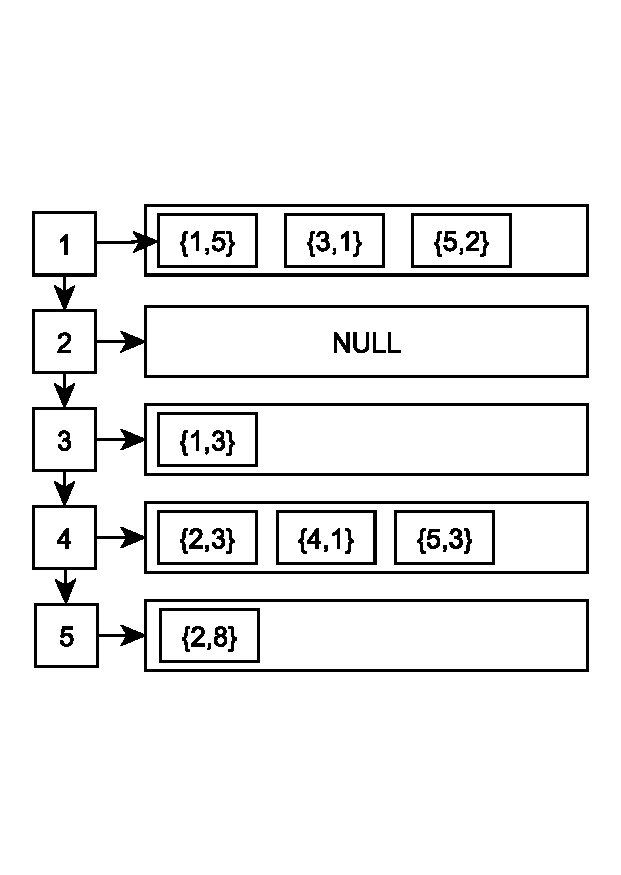
\includegraphics[width=0.5\textwidth]{file_processing.pdf}
\caption{Struktura powstała po preprocessingu}
\label{fig:preprocessing_fig}
\end{figure}

Wynikiem działania tej części preprocesingu jest struktura będąca HashMapą, zawierająca komórce $i$ liste wszystkich niezerowych elementów znajdujących się w i-tym wierszu macierzy. Figura \ref{preprocessing_fig} pokazuje fragment macierzy



\section{Dane wyświetlane}
W tym kroku preprocessingu wyliczane są informacje przydatne przy wyświetlaniu wyników. Wyliczane jest kilka pierwszych najczęściej używanych tagów przy tych dokumentach i ilość użycia tych tagów w danym dokumencie. Dodatkowo zapisana jest informacja o ilości użytkowników którzy dany dokument dodali. Zapisywane są one w tabeli w formie tekstowej w bazie danych. W czasie wyświetlania wyników, dla wybranych dokumentów dane pobierane są z wyliczone wcześniej dane i przekazywane do wyświetlenia użytkownikowi. 



\section{Mnożenie macierzy i wektorów}
\subsection{Biblioteki do mnożenia macierzy}
\subsection{Algorytm mnożenia}

\end{document}
